\documentclass[twoside]{book}

% Packages required by doxygen
\usepackage{fixltx2e}
\usepackage{calc}
\usepackage{doxygen}
\usepackage[export]{adjustbox} % also loads graphicx
\usepackage{graphicx}
\usepackage[utf8]{inputenc}
\usepackage{makeidx}
\usepackage{multicol}
\usepackage{multirow}
\PassOptionsToPackage{warn}{textcomp}
\usepackage{textcomp}
\usepackage[nointegrals]{wasysym}
\usepackage[table]{xcolor}

% Font selection
\usepackage[T1]{fontenc}
\usepackage[scaled=.90]{helvet}
\usepackage{courier}
\usepackage{amssymb}
\usepackage{sectsty}
\renewcommand{\familydefault}{\sfdefault}
\allsectionsfont{%
  \fontseries{bc}\selectfont%
  \color{darkgray}%
}
\renewcommand{\DoxyLabelFont}{%
  \fontseries{bc}\selectfont%
  \color{darkgray}%
}
\newcommand{\+}{\discretionary{\mbox{\scriptsize$\hookleftarrow$}}{}{}}

% Page & text layout
\usepackage{geometry}
\geometry{%
  a4paper,%
  top=2.5cm,%
  bottom=2.5cm,%
  left=2.5cm,%
  right=2.5cm%
}
\tolerance=750
\hfuzz=15pt
\hbadness=750
\setlength{\emergencystretch}{15pt}
\setlength{\parindent}{0cm}
\setlength{\parskip}{3ex plus 2ex minus 2ex}
\makeatletter
\renewcommand{\paragraph}{%
  \@startsection{paragraph}{4}{0ex}{-1.0ex}{1.0ex}{%
    \normalfont\normalsize\bfseries\SS@parafont%
  }%
}
\renewcommand{\subparagraph}{%
  \@startsection{subparagraph}{5}{0ex}{-1.0ex}{1.0ex}{%
    \normalfont\normalsize\bfseries\SS@subparafont%
  }%
}
\makeatother

% Headers & footers
\usepackage{fancyhdr}
\pagestyle{fancyplain}
\fancyhead[LE]{\fancyplain{}{\bfseries\thepage}}
\fancyhead[CE]{\fancyplain{}{}}
\fancyhead[RE]{\fancyplain{}{\bfseries\leftmark}}
\fancyhead[LO]{\fancyplain{}{\bfseries\rightmark}}
\fancyhead[CO]{\fancyplain{}{}}
\fancyhead[RO]{\fancyplain{}{\bfseries\thepage}}
\fancyfoot[LE]{\fancyplain{}{}}
\fancyfoot[CE]{\fancyplain{}{}}
\fancyfoot[RE]{\fancyplain{}{\bfseries\scriptsize Generated by Doxygen }}
\fancyfoot[LO]{\fancyplain{}{\bfseries\scriptsize Generated by Doxygen }}
\fancyfoot[CO]{\fancyplain{}{}}
\fancyfoot[RO]{\fancyplain{}{}}
\renewcommand{\footrulewidth}{0.4pt}
\renewcommand{\chaptermark}[1]{%
  \markboth{#1}{}%
}
\renewcommand{\sectionmark}[1]{%
  \markright{\thesection\ #1}%
}

% Indices & bibliography
\usepackage{natbib}
\usepackage[titles]{tocloft}
\setcounter{tocdepth}{3}
\setcounter{secnumdepth}{5}
\makeindex

% Hyperlinks (required, but should be loaded last)
\usepackage{ifpdf}
\ifpdf
  \usepackage[pdftex,pagebackref=true]{hyperref}
\else
  \usepackage[ps2pdf,pagebackref=true]{hyperref}
\fi
\hypersetup{%
  colorlinks=true,%
  linkcolor=blue,%
  citecolor=blue,%
  unicode%
}

% Custom commands
\newcommand{\clearemptydoublepage}{%
  \newpage{\pagestyle{empty}\cleardoublepage}%
}

\usepackage{caption}
\captionsetup{labelsep=space,justification=centering,font={bf},singlelinecheck=off,skip=4pt,position=top}

%===== C O N T E N T S =====

\begin{document}

% Titlepage & ToC
\hypersetup{pageanchor=false,
             bookmarksnumbered=true,
             pdfencoding=unicode
            }
\pagenumbering{alph}
\begin{titlepage}
\vspace*{7cm}
\begin{center}%
{\Large A\+B\+I\+A\+Web }\\
\vspace*{1cm}
{\large Generated by Doxygen 1.8.14}\\
\end{center}
\end{titlepage}
\clearemptydoublepage
\pagenumbering{roman}
\tableofcontents
\clearemptydoublepage
\pagenumbering{arabic}
\hypersetup{pageanchor=true}

%--- Begin generated contents ---
\chapter{Hierarchical Index}
\section{Class Hierarchy}
This inheritance list is sorted roughly, but not completely, alphabetically\+:\begin{DoxyCompactList}
\item \contentsline{section}{controller.\+My\+Controller}{\pageref{classcontroller_1_1_my_controller}}{}
\item \contentsline{section}{model.\+User}{\pageref{classmodel_1_1_user}}{}
\item \contentsline{section}{model.\+User\+Credential}{\pageref{classmodel_1_1_user_credential}}{}
\item \contentsline{section}{dao.\+User\+D\+AO}{\pageref{interfacedao_1_1_user_d_a_o}}{}
\begin{DoxyCompactList}
\item \contentsline{section}{dao.\+impl.\+User\+D\+A\+O\+Impl}{\pageref{classdao_1_1impl_1_1_user_d_a_o_impl}}{}
\end{DoxyCompactList}
\item \contentsline{section}{service.\+User\+Service}{\pageref{interfaceservice_1_1_user_service}}{}
\begin{DoxyCompactList}
\item \contentsline{section}{service.\+impl.\+User\+Service\+Impl}{\pageref{classservice_1_1impl_1_1_user_service_impl}}{}
\end{DoxyCompactList}
\end{DoxyCompactList}

\chapter{Class Index}
\section{Class List}
Here are the classes, structs, unions and interfaces with brief descriptions\+:\begin{DoxyCompactList}
\item\contentsline{section}{\mbox{\hyperlink{classcontroller_1_1_my_controller}{controller.\+My\+Controller}} }{\pageref{classcontroller_1_1_my_controller}}{}
\item\contentsline{section}{\mbox{\hyperlink{classmodel_1_1_user}{model.\+User}} }{\pageref{classmodel_1_1_user}}{}
\item\contentsline{section}{\mbox{\hyperlink{classmodel_1_1_user_credential}{model.\+User\+Credential}} }{\pageref{classmodel_1_1_user_credential}}{}
\item\contentsline{section}{\mbox{\hyperlink{interfacedao_1_1_user_d_a_o}{dao.\+User\+D\+AO}} }{\pageref{interfacedao_1_1_user_d_a_o}}{}
\item\contentsline{section}{\mbox{\hyperlink{classdao_1_1impl_1_1_user_d_a_o_impl}{dao.\+impl.\+User\+D\+A\+O\+Impl}} }{\pageref{classdao_1_1impl_1_1_user_d_a_o_impl}}{}
\item\contentsline{section}{\mbox{\hyperlink{interfaceservice_1_1_user_service}{service.\+User\+Service}} }{\pageref{interfaceservice_1_1_user_service}}{}
\item\contentsline{section}{\mbox{\hyperlink{classservice_1_1impl_1_1_user_service_impl}{service.\+impl.\+User\+Service\+Impl}} }{\pageref{classservice_1_1impl_1_1_user_service_impl}}{}
\end{DoxyCompactList}

\chapter{Class Documentation}
\hypertarget{classcontroller_1_1_my_controller}{}\section{controller.\+My\+Controller Class Reference}
\label{classcontroller_1_1_my_controller}\index{controller.\+My\+Controller@{controller.\+My\+Controller}}
\subsection*{Public Member Functions}
\begin{DoxyCompactItemize}
\item 
\mbox{\Hypertarget{classcontroller_1_1_my_controller_ab4548b3ff61fde48613d33bda4aa7584}\label{classcontroller_1_1_my_controller_ab4548b3ff61fde48613d33bda4aa7584}} 
void {\bfseries set\+User\+Service} (\mbox{\hyperlink{interfaceservice_1_1_user_service}{User\+Service}} user\+Service)
\item 
\mbox{\Hypertarget{classcontroller_1_1_my_controller_acb0d7ce51bc67218aaa0836fb7ba39fe}\label{classcontroller_1_1_my_controller_acb0d7ce51bc67218aaa0836fb7ba39fe}} 
\mbox{\hyperlink{interfaceservice_1_1_user_service}{User\+Service}} {\bfseries get\+User\+Service} ()
\item 
\mbox{\Hypertarget{classcontroller_1_1_my_controller_a61cacf62d1577ebd748fcba3bc3317f1}\label{classcontroller_1_1_my_controller_a61cacf62d1577ebd748fcba3bc3317f1}} 
String {\bfseries home\+Page} ()
\item 
\mbox{\Hypertarget{classcontroller_1_1_my_controller_af21c7c2ccb1b888de29c076fd0f8e7d1}\label{classcontroller_1_1_my_controller_af21c7c2ccb1b888de29c076fd0f8e7d1}} 
String {\bfseries login\+Page} (Model model)
\item 
\mbox{\Hypertarget{classcontroller_1_1_my_controller_aaf9f00246183e423f2e8b53cc9882e74}\label{classcontroller_1_1_my_controller_aaf9f00246183e423f2e8b53cc9882e74}} 
Model\+And\+View {\bfseries login\+Success} (@Valid @Model\+Attribute(\char`\"{}user\+Credential\char`\"{}) User\+Credential user\+Credential, Binding\+Result binding\+Result)
\item 
\mbox{\Hypertarget{classcontroller_1_1_my_controller_aad33f4776dfe62f8728ec601d5d4bc19}\label{classcontroller_1_1_my_controller_aad33f4776dfe62f8728ec601d5d4bc19}} 
void {\bfseries header\+Message} (Model model)
\end{DoxyCompactItemize}


The documentation for this class was generated from the following file\+:\begin{DoxyCompactItemize}
\item 
src/controller/My\+Controller.\+java\end{DoxyCompactItemize}

\hypertarget{classmodel_1_1_user}{}\section{model.\+User Class Reference}
\label{classmodel_1_1_user}\index{model.\+User@{model.\+User}}
\subsection*{Public Member Functions}
\begin{DoxyCompactItemize}
\item 
\mbox{\Hypertarget{classmodel_1_1_user_a5642dc59bf50c2e56fe30e211f319225}\label{classmodel_1_1_user_a5642dc59bf50c2e56fe30e211f319225}} 
int {\bfseries get\+Id\+User} ()
\item 
\mbox{\Hypertarget{classmodel_1_1_user_ad26c32d90f961bee59eee14631f33b3e}\label{classmodel_1_1_user_ad26c32d90f961bee59eee14631f33b3e}} 
void {\bfseries set\+Id\+User} (int id\+User)
\item 
\mbox{\Hypertarget{classmodel_1_1_user_ad5f5af7e36e8b80d2995b3ac0c226702}\label{classmodel_1_1_user_ad5f5af7e36e8b80d2995b3ac0c226702}} 
int {\bfseries get\+Id\+Role} ()
\item 
\mbox{\Hypertarget{classmodel_1_1_user_a170d0fb35bcbf315c50fd5d424c7d989}\label{classmodel_1_1_user_a170d0fb35bcbf315c50fd5d424c7d989}} 
void {\bfseries set\+Id\+Role} (int id\+Role)
\item 
\mbox{\Hypertarget{classmodel_1_1_user_a964ba13bb99d3bd7ab7c342a9c03bc46}\label{classmodel_1_1_user_a964ba13bb99d3bd7ab7c342a9c03bc46}} 
String {\bfseries get\+Username} ()
\item 
\mbox{\Hypertarget{classmodel_1_1_user_ac6fc6dcee34eafcdb9a3d05569917bbf}\label{classmodel_1_1_user_ac6fc6dcee34eafcdb9a3d05569917bbf}} 
void {\bfseries set\+Username} (String username)
\item 
\mbox{\Hypertarget{classmodel_1_1_user_ac50d8bd1c6b55d5793e22828055d5357}\label{classmodel_1_1_user_ac50d8bd1c6b55d5793e22828055d5357}} 
String {\bfseries get\+Password} ()
\item 
\mbox{\Hypertarget{classmodel_1_1_user_aea6892aee94929a724acea844061fa70}\label{classmodel_1_1_user_aea6892aee94929a724acea844061fa70}} 
void {\bfseries set\+Password} (String password)
\end{DoxyCompactItemize}


The documentation for this class was generated from the following file\+:\begin{DoxyCompactItemize}
\item 
src/model/User.\+java\end{DoxyCompactItemize}

\hypertarget{classmodel_1_1_user_credential}{}\section{model.\+User\+Credential Class Reference}
\label{classmodel_1_1_user_credential}\index{model.\+User\+Credential@{model.\+User\+Credential}}
\subsection*{Public Member Functions}
\begin{DoxyCompactItemize}
\item 
\mbox{\Hypertarget{classmodel_1_1_user_credential_a1225759d5e15cd604e89b7b0cfe50360}\label{classmodel_1_1_user_credential_a1225759d5e15cd604e89b7b0cfe50360}} 
String {\bfseries get\+Username} ()
\item 
\mbox{\Hypertarget{classmodel_1_1_user_credential_a51bd441efe07ed739e7bd2a82d25e1f1}\label{classmodel_1_1_user_credential_a51bd441efe07ed739e7bd2a82d25e1f1}} 
void {\bfseries set\+Username} (String username)
\item 
\mbox{\Hypertarget{classmodel_1_1_user_credential_ad3b213eb739ea9beb0d05acf43cfaf88}\label{classmodel_1_1_user_credential_ad3b213eb739ea9beb0d05acf43cfaf88}} 
String {\bfseries get\+Password} ()
\item 
\mbox{\Hypertarget{classmodel_1_1_user_credential_adb82e64b4ff7267fe3f059b0166c4496}\label{classmodel_1_1_user_credential_adb82e64b4ff7267fe3f059b0166c4496}} 
void {\bfseries set\+Password} (String password)
\end{DoxyCompactItemize}


The documentation for this class was generated from the following file\+:\begin{DoxyCompactItemize}
\item 
src/model/User\+Credential.\+java\end{DoxyCompactItemize}

\hypertarget{interfacedao_1_1_user_d_a_o}{}\section{dao.\+User\+D\+AO Interface Reference}
\label{interfacedao_1_1_user_d_a_o}\index{dao.\+User\+D\+AO@{dao.\+User\+D\+AO}}
Inheritance diagram for dao.\+User\+D\+AO\+:\begin{figure}[H]
\begin{center}
\leavevmode
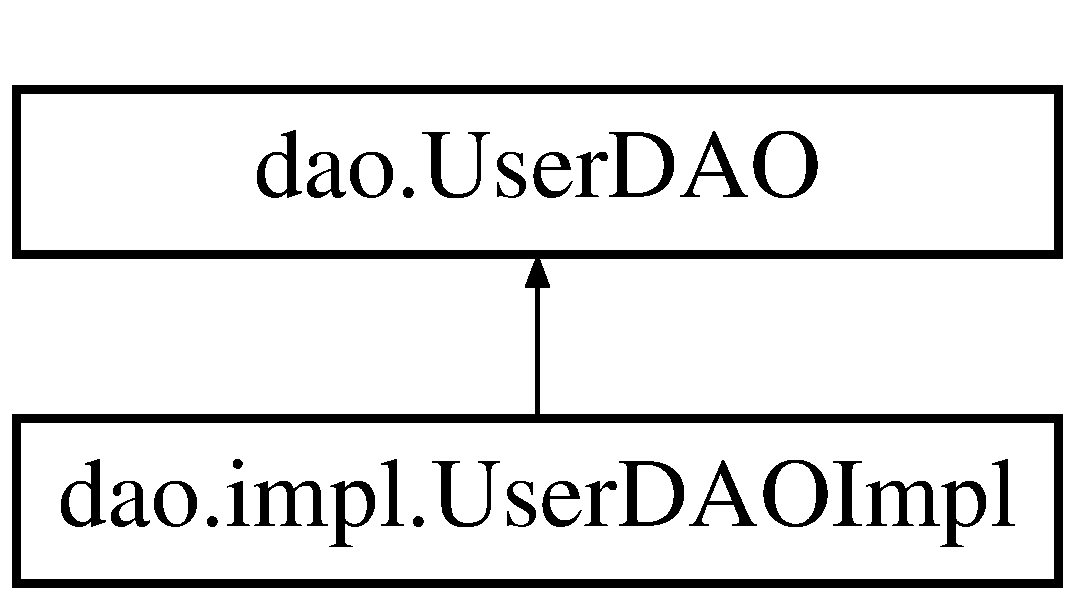
\includegraphics[height=2.000000cm]{interfacedao_1_1_user_d_a_o}
\end{center}
\end{figure}
\subsection*{Public Member Functions}
\begin{DoxyCompactItemize}
\item 
\mbox{\Hypertarget{interfacedao_1_1_user_d_a_o_ae21890f6cb21734321a991f1f0c83ed9}\label{interfacedao_1_1_user_d_a_o_ae21890f6cb21734321a991f1f0c83ed9}} 
abstract boolean {\bfseries save\+User} (\mbox{\hyperlink{classmodel_1_1_user}{User}} user)
\item 
\mbox{\Hypertarget{interfacedao_1_1_user_d_a_o_a4ff369d895891277cb1a0148039bf406}\label{interfacedao_1_1_user_d_a_o_a4ff369d895891277cb1a0148039bf406}} 
\mbox{\hyperlink{classmodel_1_1_user}{User}} {\bfseries get\+User\+Details\+By\+Username\+And\+Password} (String username, String password)
\end{DoxyCompactItemize}


The documentation for this interface was generated from the following file\+:\begin{DoxyCompactItemize}
\item 
src/dao/User\+D\+A\+O.\+java\end{DoxyCompactItemize}

\hypertarget{classdao_1_1impl_1_1_user_d_a_o_impl}{}\section{dao.\+impl.\+User\+D\+A\+O\+Impl Class Reference}
\label{classdao_1_1impl_1_1_user_d_a_o_impl}\index{dao.\+impl.\+User\+D\+A\+O\+Impl@{dao.\+impl.\+User\+D\+A\+O\+Impl}}
Inheritance diagram for dao.\+impl.\+User\+D\+A\+O\+Impl\+:\begin{figure}[H]
\begin{center}
\leavevmode
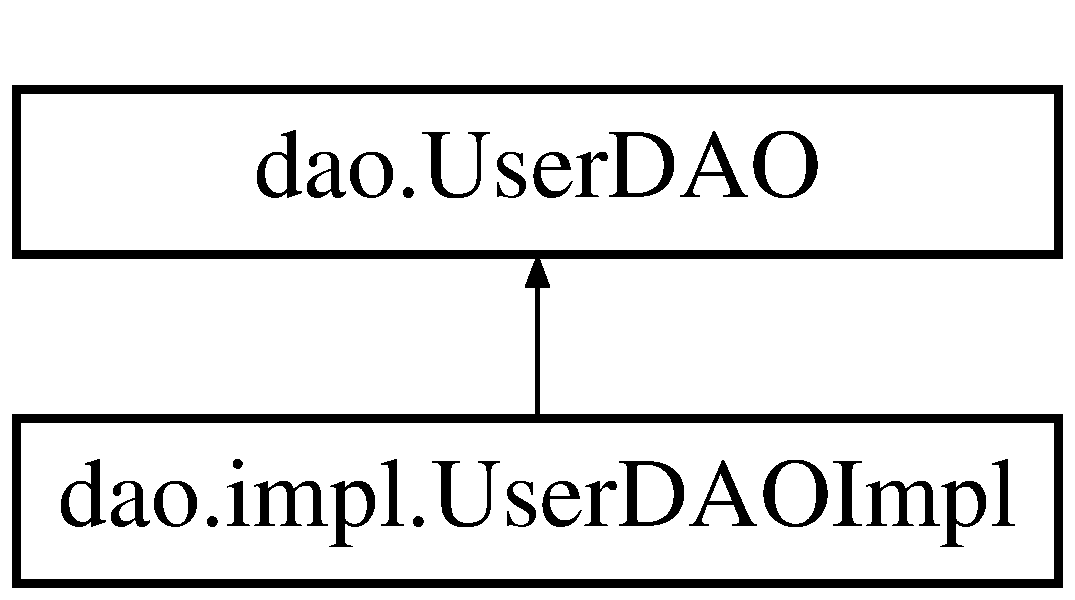
\includegraphics[height=2.000000cm]{classdao_1_1impl_1_1_user_d_a_o_impl}
\end{center}
\end{figure}
\subsection*{Public Member Functions}
\begin{DoxyCompactItemize}
\item 
\mbox{\Hypertarget{classdao_1_1impl_1_1_user_d_a_o_impl_a73d10aae918da3e5de10052c3b36665c}\label{classdao_1_1impl_1_1_user_d_a_o_impl_a73d10aae918da3e5de10052c3b36665c}} 
void {\bfseries set\+Hibernate\+Template} (Hibernate\+Template hibernate\+Template)
\item 
\mbox{\Hypertarget{classdao_1_1impl_1_1_user_d_a_o_impl_acf4d0494ed9bb7d9dd049f1ea10328a4}\label{classdao_1_1impl_1_1_user_d_a_o_impl_acf4d0494ed9bb7d9dd049f1ea10328a4}} 
Hibernate\+Template {\bfseries get\+Hibernate\+Template} ()
\item 
\mbox{\Hypertarget{classdao_1_1impl_1_1_user_d_a_o_impl_a859e94509e4fb4372be8e0e2fa2ab4ab}\label{classdao_1_1impl_1_1_user_d_a_o_impl_a859e94509e4fb4372be8e0e2fa2ab4ab}} 
boolean {\bfseries save\+User} (\mbox{\hyperlink{classmodel_1_1_user}{User}} user)
\item 
\mbox{\Hypertarget{classdao_1_1impl_1_1_user_d_a_o_impl_a15e2d9e735ce7d780024e14fe735c7e9}\label{classdao_1_1impl_1_1_user_d_a_o_impl_a15e2d9e735ce7d780024e14fe735c7e9}} 
\mbox{\hyperlink{classmodel_1_1_user}{User}} {\bfseries get\+User\+Details\+By\+Username\+And\+Password} (String username, String password)
\end{DoxyCompactItemize}


The documentation for this class was generated from the following file\+:\begin{DoxyCompactItemize}
\item 
src/dao/impl/User\+D\+A\+O\+Impl.\+java\end{DoxyCompactItemize}

\hypertarget{interfaceservice_1_1_user_service}{}\section{service.\+User\+Service Interface Reference}
\label{interfaceservice_1_1_user_service}\index{service.\+User\+Service@{service.\+User\+Service}}
Inheritance diagram for service.\+User\+Service\+:\begin{figure}[H]
\begin{center}
\leavevmode
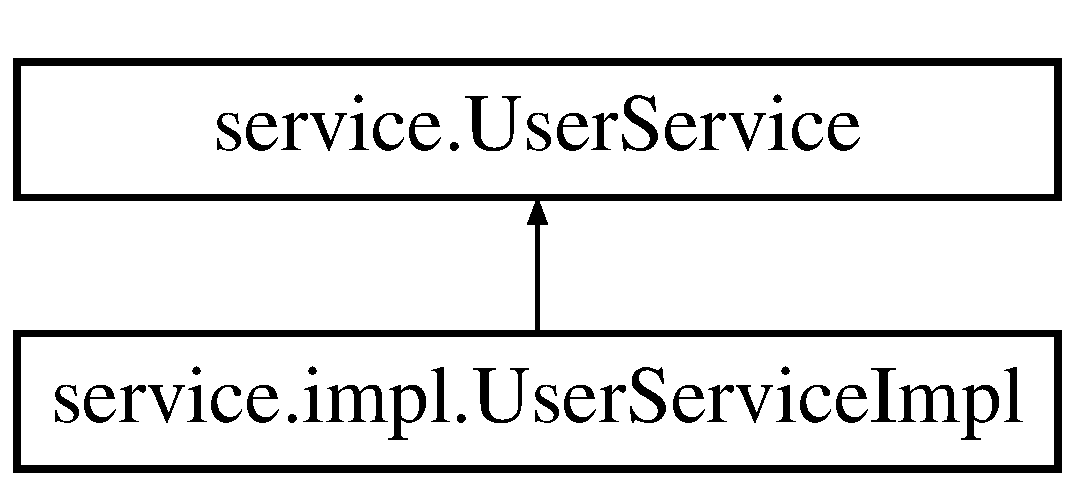
\includegraphics[height=2.000000cm]{interfaceservice_1_1_user_service}
\end{center}
\end{figure}
\subsection*{Public Member Functions}
\begin{DoxyCompactItemize}
\item 
\mbox{\Hypertarget{interfaceservice_1_1_user_service_a34e74aa724e499073f3c3051e8ff8e42}\label{interfaceservice_1_1_user_service_a34e74aa724e499073f3c3051e8ff8e42}} 
abstract \mbox{\hyperlink{classmodel_1_1_user}{User}} {\bfseries validate\+User\+Credential} (String username, String password)
\item 
\mbox{\Hypertarget{interfaceservice_1_1_user_service_a111804c2062b3d6f948ef550051a5ad3}\label{interfaceservice_1_1_user_service_a111804c2062b3d6f948ef550051a5ad3}} 
abstract boolean {\bfseries register\+User} (\mbox{\hyperlink{classmodel_1_1_user}{User}} user)
\end{DoxyCompactItemize}


The documentation for this interface was generated from the following file\+:\begin{DoxyCompactItemize}
\item 
src/service/User\+Service.\+java\end{DoxyCompactItemize}

\hypertarget{classservice_1_1impl_1_1_user_service_impl}{}\section{service.\+impl.\+User\+Service\+Impl Class Reference}
\label{classservice_1_1impl_1_1_user_service_impl}\index{service.\+impl.\+User\+Service\+Impl@{service.\+impl.\+User\+Service\+Impl}}
Inheritance diagram for service.\+impl.\+User\+Service\+Impl\+:\begin{figure}[H]
\begin{center}
\leavevmode
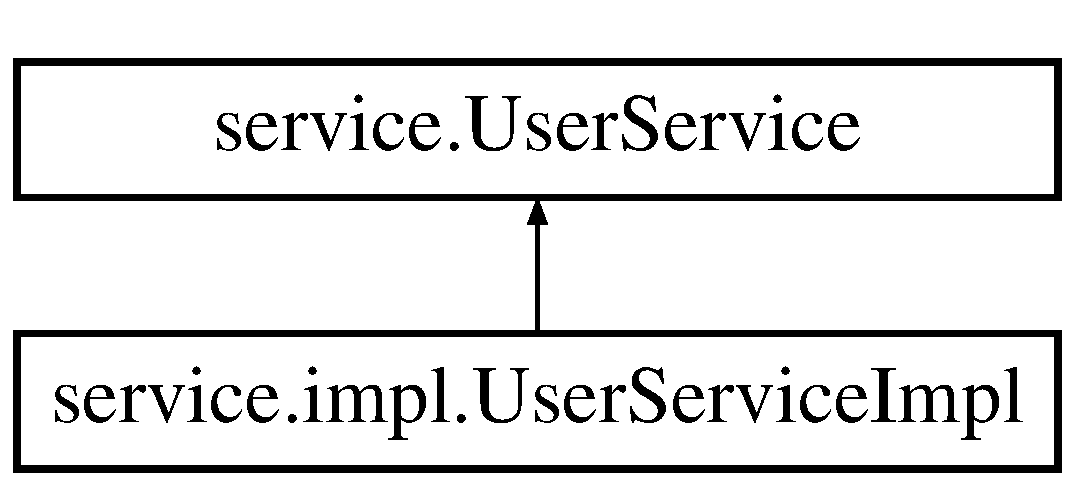
\includegraphics[height=2.000000cm]{classservice_1_1impl_1_1_user_service_impl}
\end{center}
\end{figure}
\subsection*{Public Member Functions}
\begin{DoxyCompactItemize}
\item 
\mbox{\Hypertarget{classservice_1_1impl_1_1_user_service_impl_af730727180fc704b8c0a0b8849431012}\label{classservice_1_1impl_1_1_user_service_impl_af730727180fc704b8c0a0b8849431012}} 
void {\bfseries set\+User\+D\+AO} (\mbox{\hyperlink{interfacedao_1_1_user_d_a_o}{User\+D\+AO}} user\+D\+AO)
\item 
\mbox{\Hypertarget{classservice_1_1impl_1_1_user_service_impl_a35d326db6a04cdaf680d59ecfcf1a887}\label{classservice_1_1impl_1_1_user_service_impl_a35d326db6a04cdaf680d59ecfcf1a887}} 
\mbox{\hyperlink{interfacedao_1_1_user_d_a_o}{User\+D\+AO}} {\bfseries get\+User\+D\+AO} ()
\item 
\mbox{\Hypertarget{classservice_1_1impl_1_1_user_service_impl_a11d9956ff2936f4541b17d3dd5780ba4}\label{classservice_1_1impl_1_1_user_service_impl_a11d9956ff2936f4541b17d3dd5780ba4}} 
boolean {\bfseries register\+User} (\mbox{\hyperlink{classmodel_1_1_user}{User}} user)
\item 
\mbox{\Hypertarget{classservice_1_1impl_1_1_user_service_impl_a13ad8f7d06c99cb7d2906fd8536ad37f}\label{classservice_1_1impl_1_1_user_service_impl_a13ad8f7d06c99cb7d2906fd8536ad37f}} 
\mbox{\hyperlink{classmodel_1_1_user}{User}} {\bfseries validate\+User\+Credential} (String username, String password)
\end{DoxyCompactItemize}


The documentation for this class was generated from the following file\+:\begin{DoxyCompactItemize}
\item 
src/service/impl/User\+Service\+Impl.\+java\end{DoxyCompactItemize}

%--- End generated contents ---

% Index
\backmatter
\newpage
\phantomsection
\clearemptydoublepage
\addcontentsline{toc}{chapter}{Index}
\printindex

\end{document}
